% =========================================================
% KHAI BÁO CẤU HÌNH (PREAMBLE)
% =========================================================
\documentclass[aspectratio=169, 9pt]{beamer}

% Load theme HUST (nhớ để file beamerthemeHUST.sty cùng thư mục)
\usetheme[theme=blue,logo=logowithtextvi]{HUST} 

% Các package cần thiết
\usepackage[T5]{fontenc} % Hỗ trợ tiếng Việt
\usepackage[utf8]{inputenc}
\usepackage{lmodern}     
\usepackage{enumitem}    
\usepackage{tcolorbox}   
\usepackage{listings}    
\usepackage{verbatim}
\usepackage{amsmath}
\usepackage[table]{xcolor}
\usepackage{tikz}
\usetikzlibrary{positioning,arrows.meta,calc}
\usepackage{minted}

% \usetikzlibrary{decorations.pathreplacing,arrows.meta}
\tcbuselibrary{listingsutf8, skins, minted}

% Định nghĩa lệnh đặt nội dung tự do
\newcommand{\placecontent}[4]{%
  \tikz[remember picture,overlay]
    \node[anchor=north west]
      at ([xshift=#1,yshift=-#2]current page.north west)
      {\parbox{#3}{#4}};
}

% Thông tin metadata
\title{LẬP TRÌNH C CƠ BẢN}
\author{SoICT - HUST}
\date{}

% Chỉnh footer hiện số trang
\setbeamertemplate{footline}{%
  \hfill%
  \insertframenumber\hspace{0.5cm}\vspace{0.3cm}
}

% =========================================================
% NỘI DUNG CHÍNH (BODY)
% =========================================================
\begin{document}

% --- TRANG 1: BRAND SLIDE (Trang bìa HUST) ---
\HUSTInsertBrandSlide

% --- TRANG 2: TÊN BÀI HỌC ---
{
\HUSTUseBackground{onelove.pdf}
\begin{frame}
  \ifdefstring{\insertaspectratio}{169}{
    % Logo góc
    \HUSTCornerImage{assets/logo/04.pdf}

    % Tên môn học
    \placecontent{0.5cm}{0.33\paperheight}{0.85\paperwidth}{
        \color{\HUSTFrameTitleTextColor}\bfseries\fontsize{22pt}{30pt}\selectfont
        LẬP TRÌNH C CƠ BẢN
    }
    
    % Tên bài học
    \placecontent{0.5cm}{0.60\paperheight}{0.8\paperwidth}{
        \color{\HUSTFrameTitleTextColor}\fontsize{14pt}{18pt}\selectfont
        Kiểu dữ liệu cơ bản, vào ra file
    }
  }{}
\end{frame}
}

% --- TRANG 3: NỘI DUNG ---
% Đã xóa lệnh \HUSTInsertThemeSlide để không bị thừa trang
% Slide này sẽ tự động dùng background mặc định (trắng + thanh header/footer)

\begin{frame}{Nội dung}
    \begin{itemize}[label={\tiny$\bullet$}, itemsep=1em] 
        \item Giới thiệu về môn học
        \item Ôn tập về C
        \begin{itemize}[label={\tiny$\bullet$}, itemsep=0.5em]
            \item Mảng
            \item Xâu ký tự
            \item Con trỏ
            \item Tham số dòng lệnh
        \end{itemize}
    \end{itemize}
\end{frame}

% --- SLIDE 4: CHUYỂN MỤC (SECTION SLIDE) ---
% PDF Page 4: "Nội dung môn học"
% Đã fix: Đẩy text sang phải (né phần xanh), chỉnh màu đỏ HUST, font vừa phải
{
\HUSTUseBackground{theme_hust_oneside.pdf}
\begin{frame}
    % 0.38\paperwidth: Đẩy sang phải khoảng 40% màn hình để vào phần trắng
    \placecontent{0.38\paperwidth}{0.45\paperheight}{0.6\paperwidth}{
        \centering
        \color{HUSTRed}\bfseries\fontsize{24pt}{30pt}\selectfont
        NỘI DUNG MÔN HỌC
    }
\end{frame}
}

% Định nghĩa Section (giúp tạo mục lục nếu cần sau này)
\section{Giới thiệu về môn học}

% --- SLIDE 5: GIỚI THIỆU MÔN HỌC (1) ---
% PDF Page 5: Mục tiêu, mức độ...
% Đã fix: Đổi bullet thành dấu chấm tròn (bullet) giống ảnh PDF gốc
\begin{frame}{Giới thiệu về môn học}
    \begin{itemize}[label=$\bullet$, itemsep=1em] % Dùng dấu chấm tròn, dãn dòng 1em cho thoáng
        \item Thực hành lập trình theo các chủ đề về cấu trúc dữ liệu và giải thuật
        \begin{itemize}[label=$\circ$, itemsep=0.5em] % Level 2 dùng tròn rỗng
            \item Mức độ: cơ sở
            \item Cài đặt các cấu trúc dữ liệu – thuật toán
            \item Ứng dụng vào giải quyết một số bài toán thực tế.
        \end{itemize}
        \item Ngôn ngữ lập trình: \textbf{C}
    \end{itemize}
\end{frame}

% --- SLIDE 6: GIỚI THIỆU MÔN HỌC (2) ---
% PDF Page 6: Môi trường, công cụ
% Đã fix: Layout nhất quán với trang 5
\begin{frame}{Giới thiệu về môn học}
    \begin{itemize}[label=$\bullet$, itemsep=1em]
        \item Môi trường khuyến nghị:
        \begin{itemize}[label=$\circ$, itemsep=0.8em]
            \item Hệ điều hành UNIX
        \end{itemize}
        \item Chương trình dịch: \texttt{gcc}
        \item Chương trình soạn thảo mã nguồn: Emacs, K-Developer.
    \end{itemize}
\end{frame}

% --- SLIDE 7: ĐÁNH GIÁ KẾT QUẢ ---
% PDF Page 7: Cơ chế chấm điểm (30% - 70%)
\begin{frame}{Đánh giá kết quả môn học}
    \begin{itemize}[label=$\bullet$, itemsep=1em]
        \item Điểm quá trình: \textbf{30\%}
        \begin{itemize}[label=$\circ$, itemsep=0.5em]
            \item Chấm điểm bài tập về nhà hàng tuần, kết hợp với chất lượng hoàn thành thực hành trên lớp.
            \item Mỗi tuần: 4, 5 sinh viên.
        \end{itemize}
        \item Cuối kỳ: \textbf{70\%}
        \begin{itemize}[label=$\circ$, itemsep=0.5em]
            \item Thi lập trình trên máy tính.
            \item Điểm đánh giá dựa trên kết quả chạy chương trình, không đánh giá dựa trên mã nguồn.
        \end{itemize}
    \end{itemize}
\end{frame}

% --- SLIDE 8: CHUYỂN MỤC (SECTION SLIDE) ---
% PDF Page 8: "Ôn tập về C"
% Layout giống trang 4 (Nội dung môn học)
{
\HUSTUseBackground{theme_hust_oneside.pdf}
\begin{frame}
    % Căn lề phải giống trang 4 bro vừa sửa
    \placecontent{0.38\paperwidth}{0.45\paperheight}{0.6\paperwidth}{
        \centering
        \color{HUSTRed}\bfseries\fontsize{30pt}{30pt}\selectfont
        ÔN TẬP VỀ C
    }
\end{frame}
}

\section{Ôn tập về C}

% --- SLIDE 9: CÚ PHÁP GCC ---
% PDF Page 9: Các flag gcc và ví dụ lệnh
% Dùng [fragile] để chứa code block
\begin{frame}[fragile]{Cú pháp dịch chương trình bằng gcc}
    \begin{itemize}[label=$\bullet$, itemsep=0.5em]
        \item Các tham số:
        \begin{itemize}[label=$\bullet$, itemsep=0.3em]
            \item \texttt{-Wall} : bật tất cả các cảnh báo
            \item \texttt{-c}: tạo tập tin object
            \item \texttt{-o}: tạo tập tin chương trình
            \item \texttt{-g}: thêm thông tin gỡ rối
            \item \texttt{-l}: sử dụng kèm thư viện
        \end{itemize}
    \end{itemize}

    \vspace{0.5em}
    
    % Box code command line (Giống style terminal)
    \begin{tcolorbox}[colback=gray!10, colframe=black, boxrule=0.5pt, width=0.9\textwidth, arc=2pt, left=5pt]
        \ttfamily\small
        > gcc -Wall hello.c -o runhello \\
        > ./runhello
    \end{tcolorbox}

\end{frame}

% --- SLIDE 10: CHỦ ĐỀ ---
% PDF Page 10: Liệt kê các nội dung chi tiết
\begin{frame}{Chủ đề}
    \begin{itemize}[label=$\bullet$, itemsep=0.8em]
        \item Ôn tập về các kiểu dữ liệu:
        \begin{itemize}[label=$\bullet$, itemsep=0.4em]
            \item mảng,
            \item xâu ký tự,
            \item con trỏ.
        \end{itemize}
        \item Xây dựng chương trình với đối số dòng lệnh
        \item Thao tác với tập tin văn bản
        \begin{itemize}[label=$\bullet$, itemsep=0.4em]
            \item Đọc ghi tập tin theo từng ký tự
            \item Đọc ghi tập tin theo từng dòng
            \item Đọc ghi tập tin theo đặc tả định dạng
        \end{itemize}
        \item Các bài tập lập trình
    \end{itemize}
\end{frame}

% --- SLIDE 11: CHUYỂN MỤC (SECTION SLIDE) ---
% PDF Page 11: "Mảng - Array"
% Vẫn giữ layout lệch phải cho đồng bộ với các trang trước
{
\HUSTUseBackground{theme_hust_oneside.pdf}
\begin{frame}
    \placecontent{0.38\paperwidth}{0.45\paperheight}{0.6\paperwidth}{
        \centering
        \color{HUSTRed}\bfseries\fontsize{30pt}{30pt}\selectfont
        Mảng - Array
    }
\end{frame}
}

\section{Mảng}

% --- SLIDE 12: ĐỊNH NGHĨA MẢNG ---
% PDF Page 12: Khái niệm và ví dụ
\begin{frame}{I. Mảng}
    \begin{itemize}[label=$\bullet$, itemsep=1em]
        \item Khối liên tục các biến cùng kiểu dữ liệu, cùng tên
        \item Mảng có thể khai báo với bất cứ kiểu dữ liệu nào
        \begin{itemize}[label=$\bullet$, itemsep=0.5em]
            \item VD: \texttt{int A[10];} là khai báo mảng 10 số nguyên.
        \end{itemize}
        \item Các ví dụ về sử dụng mảng:
        \begin{itemize}[label=$\bullet$, itemsep=0.5em]
            \item Danh sách điểm của các sinh viên
            \item Dãy số nhập từ người dùng
            \item Véc tơ
            \item Ma trận
        \end{itemize}
    \end{itemize}
\end{frame}

% --- SLIDE 13: MẢNG TRONG BỘ NHỚ (TIKZ FINAL FIX) ---
\begin{frame}[fragile]{Mảng trong bộ nhớ trong}
    \begin{itemize}[label=$\bullet$, itemsep=0.8em]
        \item Dãy liên tục các biến cùng kiểu, nằm kế tiếp nhau
        \item Tên mảng chứa địa chỉ bộ nhớ của phần tử đầu tiên
        \item Ví dụ: \texttt{double S[10];}
    \end{itemize}

    \vspace{0.5cm}

    \begin{center}
        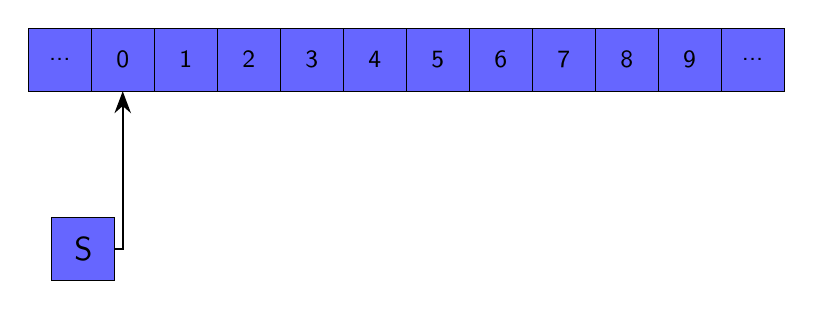
\begin{tikzpicture}[
            node distance=0pt,
            outer sep=0pt,
            % Style cho các ô nhớ
            cell/.style={
                draw=black,
                fill=blue!60!white, 
                minimum width=0.8cm,
                minimum height=0.8cm,
                text=black,
                font=\sffamily\small,
                anchor=west
            },
            % Style cho con trỏ S
            ptr/.style={
                draw=black,
                fill=blue!60!white,
                minimum width=0.8cm,
                minimum height=0.8cm,
                text=black,
                font=\sffamily\large
            }
        ]
            % HÀNG 1: DÃY Ô NHỚ
            \node[cell] (start) {...};
            % Các ô tiếp theo xếp liền kề nhau
            \node[cell] (n0) at (start.east) {0};
            \node[cell] (n1) at (n0.east) {1};
            \node[cell] (n2) at (n1.east) {2};
            \node[cell] (n3) at (n2.east) {3};
            \node[cell] (n4) at (n3.east) {4};
            \node[cell] (n5) at (n4.east) {5};
            \node[cell] (n6) at (n5.east) {6};
            \node[cell] (n7) at (n6.east) {7};
            \node[cell] (n8) at (n7.east) {8};
            \node[cell] (n9) at (n8.east) {9};
            \node[cell] (end) at (n9.east) {...};

            % HÀNG 2: S NẰM DƯỚI Ô "..." VÀ DỊCH TRÁI MỘT CHÚT
            \node[ptr] (S) at ($(n0.south)+(-0.5cm,-2cm)$) {S};

            % MŨI TÊN VUÔNG GÓC (L-SHAPE)
            % Đi từ cạnh phải S -> Sang phải -> Lên đáy ô 0
            \draw[-{Stealth[scale=1.2]}, thick] (S.east) -| (n0.south);

        \end{tikzpicture}
    \end{center}

    \vspace{0.2cm}
    \begin{itemize}[label=$\bullet$]
        \item Phần tử thứ $k$ của mảng $A$ truy cập qua chỉ số: $A[k-1]$ (bắt đầu từ 0)
    \end{itemize}
\end{frame}

% --- SLIDE 14: VÍ DỤ ĐẢO NGƯỢC ---
\begin{frame}[fragile]{Ví dụ - hiển thị mảng theo chiều ngược}
    \begin{columns}[T]
        % Cột trái: Đề bài
        \begin{column}{0.4\textwidth}
            \textbf{Ví dụ 1.}
            \vspace{0.5em}
            \begin{itemize}[label=$\bullet$, leftmargin=1em, itemsep=0.8em]
                \item Viết chương trình nhập vào 1 mảng 10 số thực từ bàn phím và in ra các giá trị vừa nhập theo thứ tự đảo ngược.
                \item Các giá trị in ra lấy tới 4 chữ số thập phân.
            \end{itemize}
        \end{column}

        % Cột phải: Code
        \begin{column}{0.58\textwidth}
            % Style đồng bộ Week 2: Box trắng, viền đen, bo góc nhẹ
            \begin{tcblisting}{
                colback=white, 
                colframe=black, 
                boxrule=0.5pt, 
                arc=2pt,
                listing engine=minted, 
                minted language=c,
                minted options={
                    fontsize=\scriptsize, 
                    breaklines, 
                    autogobble, 
                    baselinestretch=1,
                    tabsize=4
                },
                listing only,
                left=2mm, top=2mm, bottom=2mm
            }
#include <stdio.h>

int main(void) {
    int i; 
    double A[10];
    
    printf("Please enter 10 numbers:\n");
    for (i = 0; i < 10; i++)
        scanf("%lf", &A[i]);
        
    printf("Numbers in reversed order:\n");
    for (i = 9; i >= 0; i--)
        printf("%0.4f\n", A[i]);
        
    return 0;
}
            \end{tcblisting}
        \end{column}
    \end{columns}
\end{frame}

% --- SLIDE 15: BÀI TẬP ỨNG DỤNG 1 (ĐÃ FIX LỖI MEMORY) ---
% Fix: Thay enumerate bằng itemize với nhãn thủ công để tránh xung đột package
\begin{frame}{Bài tập ứng dụng}
    \begin{itemize}[label=$\bullet$, itemsep=0.8em]
        \item \textbf{Bài tập 1.} Với danh sách các phần tử đã nhập trong Ví dụ 1, hãy in ra (các) phần tử có giá trị gần nhất với giá trị trung bình các phần tử của dãy.
        
        \item \textbf{Gợi ý:}
        % Dùng itemize nhưng set nhãn là số 1. 2. 3.
        \begin{itemize}[itemsep=0.5em] 
            \item[\textbf{1.}] Tính giá trị trung bình dãy - \texttt{average}
            \item[\textbf{2.}] Duyệt dãy, so sánh giá trị lệch của các phần tử với giá trị trung bình \texttt{average}. Ghi nhận giá trị chênh lệch nhỏ nhất là \texttt{mindiff}.
            \item[\textbf{3.}] Duyệt lại dãy lần nữa, in ra các phần tử có giá trị chênh lệch so với \texttt{average} bằng \texttt{mindiff}.
        \end{itemize}
        
        \item \textbf{Chú ý:}
        \begin{itemize}[label=$\bullet$]
            \item Mảng số thực có sự sai số do làm tròn nên nếu cần chuyển về số nguyên và chấp nhận sai số.
            \item $0.2 + 0.1$ Không bằng $0.3$
        \end{itemize}
    \end{itemize}
\end{frame}

% --- SLIDE 16 (FINAL FIX): BÀI TẬP 2 ---
\begin{frame}{Bài tập ứng dụng}
    \begin{itemize}[label=$\bullet$]
        \item \textbf{Bài tập 2.} Viết chương trình nhập vào 1 xâu ký tự chỉ gồm các ký tự chữ thường. Hãy in ra tần số xuất hiện của các ký tự chữ cái trong xâu, bỏ qua các ký tự không phải chữ cái.
    \end{itemize}
    
    \vspace{0.5cm}

    \begin{columns}[T]
        % Cột trái: Gợi ý (Đẩy xuống một chút cho cân với box bên phải)
        \begin{column}{0.55\textwidth}
            \textbf{Gợi ý:}
            \begin{itemize}[label=$\bullet$, itemsep=0.5em]
                \item Dùng mảng để đếm tần số xuất hiện các ký tự chữ cái.
                \item Có 26 ký tự chữ cái thường, mảng \texttt{int count[26]}.
                \item Ký tự 'a' tương ứng với phần tử đầu mảng chỉ số 0.
                \item Đọc vào xâu bằng cách đọc vào từng ký tự như mảng hoặc dùng hàm có sẵn trong thư viện string.
            \end{itemize}
        \end{column}

        % Cột phải: Box kết quả (Clean style)
        \begin{column}{0.45\textwidth}
            % Box trắng viền đen, không fill màu tiêu đề
            \begin{tcolorbox}[colback=white, colframe=black, boxrule=0.8pt, arc=0pt, left=3pt, right=3pt, top=3pt, bottom=3pt]
                \small
                Kết quả hiển thị với xâu đầu vào: "hello, world!"
                \vspace{0.2cm}
                \hrule % Đường kẻ ngang mỏng phân cách
                \vspace{0.2cm}
                
                \scriptsize
                The letter 'd' appears 1 time(s).\\
                The letter 'e' appears 1 time(s).\\
                The letter 'h' appears 1 time(s).\\
                The letter 'l' appears 3 time(s).\\
                The letter 'o' appears 2 time(s).\\
                The letter 'r' appears 1 time(s).\\
                The letter 'w' appears 1 time(s).
            \end{tcolorbox}
        \end{column}
    \end{columns}
\end{frame}

% --- SLIDE 17: BÀI TẬP 2 (LỜI GIẢI 1) ---
\begin{frame}[fragile]{Bài tập ứng dụng}
    % Sử dụng tcblisting chuẩn style Week 2
    \begin{tcblisting}{
        colback=white, 
        colframe=black, 
        boxrule=0.5pt, 
        arc=2pt,
        listing engine=minted, 
        minted language=c,
        minted options={
            fontsize=\scriptsize, 
            breaklines, 
            autogobble, 
            baselinestretch=0.95, % Giảm nhẹ giãn dòng để code vừa khít slide
            tabsize=4
        },
        listing only,
        left=2mm, top=2mm, bottom=2mm
    }
#include <stdio.h>
// maximum size 26
#define ALPHABET_LEN 26

int main(void) {
    int i = 0, count[ALPHABET_LEN] = {0}; // initialize all elements to zero
    char c = '\0';
    
    printf("Please enter a line of text: \n");
    /* Read in letter by letter and update the count array */
    c = getchar();
    while (c != '\n' && c >= 0) {
        if (c <= 'z' && c >= 'a')
            ++count[c - 'a'];
        if (c <= 'Z' && c >= 'A')
            ++count[c - 'A'];
        c = getchar();
    }

    for (i = 0; i < ALPHABET_LEN; ++i) {
        if (count[i] > 0)
            printf("The letter '%c' appears %d time(s).\n", 'a' + i, count[i]);
    }
    return 0;
}
    \end{tcblisting}
\end{frame}

% --- SLIDE 18: BÀI TẬP 2 (LỜI GIẢI 2) ---
\begin{frame}[fragile]{Bài tập ứng dụng}
    \begin{tcblisting}{
        colback=white, 
        colframe=black, 
        boxrule=0.5pt, 
        arc=2pt,
        listing engine=minted, 
        minted language=c,
        minted options={
            fontsize=\scriptsize, 
            breaklines, 
            autogobble, 
            baselinestretch=0.95,
            tabsize=4
        },
        listing only,
        left=2mm, top=2mm, bottom=2mm
    }
#include <stdio.h>
#include <string.h>
#define ALPHABET_LEN 26

int main() {
    int i = 0, count[ALPHABET_LEN] = {0};
    char s[20], c = '\0';

    printf("Please enter a line of text: \n");
    gets(s);

    for (i = 0; i < strlen(s); i++) {
        c = s[i];
        if (c <= 'z' && c >= 'a') {
            ++count[c - 'a'];
        }
    }

    for (i = 0; i < ALPHABET_LEN; ++i) {
        if (count[i] > 0) {
            printf("The letter '%c' appears %d time(s).\n", 'a' + i, count[i]);
        }
    }
    return 0;
}
    \end{tcblisting}
\end{frame}

% --- SLIDE 19: BÀI TẬP 3 (ĐỀ BÀI) ---
% Cập nhật nội dung theo yêu cầu: Bổ sung ví dụ thứ tự mảng
\begin{frame}{Bài tập ứng dụng}
    \small % Giữ font nhỏ vừa mắt
    \begin{itemize}[label=$\bullet$, itemsep=0.8em]
        \item \textbf{Bài tập 3.} Viết chương trình dạng hàm:
        \begin{itemize}[label=$\circ$, itemsep=0.5em]
            \item Hàm so sánh 2 mảng (có cùng số lượng phần tử) xem có trùng nhau (các phần tử ở cùng vị trí giống nhau).
            \item Nếu 2 mảng trùng nhau thì trả về giá trị 1, và 0 nếu ngược lại.
            \item Hàm kiểm tra 2 mảng (có cùng phần tử) có trùng nhau (mở rộng). Hai mảng sẽ chứa các phần tử như nhau, nhưng các phần tử lúc này không cần ở vị trí giống nhau.
            \item[] \textit{VD:} Mảng $A=\{2,4,4,5\}$ trùng với $B=\{4,5,4,2\}$ nhưng không trùng với $C=\{5,5,4,2\}$.
            
            \item Hàm kiểm tra 2 mảng (có cùng phần tử) các phần tử liên tiếp có cùng thứ tự hay không.
            \item[] \textit{VD:} Mảng $A$ mà $A[i] \le A[i+1]$ thì trong mảng $B$ cũng phải tương tự $B[i] \le B[i+1]$.
            \item[] $A=\{1,3,2,7\}$ sẽ cùng thứ tự với $B=\{2,7,3,4\}$.
        \end{itemize}
    \end{itemize}
\end{frame}

% --- SLIDE 20: CODE BÀI TẬP 3 (MINTED + OVERLAP FIX) ---
\begin{frame}[fragile]{Bài tập ứng dụng}
    % Dùng TikZ để căn chỉnh vị trí 2 box đè lên nhau
    \begin{tikzpicture}[remember picture, overlay]
        
        % BOX 1: Hàm compare_arrays (Nằm ở góc trên bên trái)
        \node[anchor=north west] at ([xshift=0.5cm, yshift=-1.5cm]current page.north west) {
            \begin{tcolorbox}[colback=white, colframe=black, width=0.6\paperwidth, boxrule=0.5pt, arc=2pt]
% Code Box 1 dùng minted
\begin{minted}[fontsize=\tiny, breaklines, baselinestretch=1]{c}
#include <stdio.h>
#define SIZE 5

/*function check if two arays are identical*/
int compare_arrays(int arr1[], int arr2[], int size) {
    int i = 0;
    for (i = 0; i < size; ++i) {
        if (arr1[i] != arr2[i])
            return 0;
    }
    return 1;
}
\end{minted}
            \end{tcolorbox}
        };

        % BOX 2: Hàm main (Nằm ở góc dưới bên phải, đè lên Box 1)
        % Đã dịch lên 1cm (0.3cm -> 1.3cm) theo yêu cầu
        \node[anchor=south east] at ([xshift=-0.5cm, yshift=1.3cm]current page.south east) {
            % Thêm shadow đen nhạt để nhìn rõ hiệu ứng đè lên nhau
            \begin{tcolorbox}[colback=white, colframe=black, width=0.65\paperwidth, boxrule=0.5pt, arc=2pt, shadow={2mm}{-2mm}{0mm}{black!30}]
% Code Box 2 dùng minted
\begin{minted}[fontsize=\tiny, breaklines, baselinestretch=1]{c}
int main(void) {
    int input1[SIZE], input2[SIZE], i;

    printf("Please enter a list of %d integers:\n", SIZE);
    for (i = 0; i < SIZE; ++i) scanf("%d", &input1[i]);

    printf("Please enter another list of %d integers:\n", SIZE);
    for (i = 0; i < SIZE; ++i) scanf("%d", &input2[i]);

    if (compare_arrays(input1, input2, SIZE) == 1)
        printf("Both lists are identical!\n");
    else
        printf("The lists are not identical...\n");
    return 0;
}
\end{minted}
            \end{tcolorbox}
        };

    \end{tikzpicture}
\end{frame}

% --- SLIDE 21: LAB TEST 01 ---
% Bài tìm số chính phương
\begin{frame}[fragile]{Lab test}
    \small
    \textbf{Lab 01. Find all perfect square in a sequence}
    \vspace{0.3cm}
    \begin{itemize}[label=$\bullet$, itemsep=0.5em]
        \item Given a sequence of $n$ integers $a_1, a_2, ..., a_n$. Compute the number $Q$ of perfect squares (the number of type $a^2$) of that sequence.
        \item \textbf{Input:}
        \begin{itemize}[label=-]
            \item Line 1: contains a positive integer $n$ ($1 \leq n \leq 100000$)
            \item Line 2: contains $n$ positive integer $a_1, a_2, ..., a_n$ ($1 \leq a_i \leq 1000000$)
        \end{itemize}
        \item \textbf{Output:} Write the value $Q$
    \end{itemize}

    \vspace{0.4cm}
    % Bảng ví dụ Input/Output gọn gàng
    \begin{table}
        \centering
        \small
        \begin{tabular}{|p{0.4\textwidth}|p{0.2\textwidth}|}
            \hline
            \textbf{Input} & \textbf{Output} \\
            \hline
            \texttt{5} \newline \texttt{3 2 4 7 9} & \texttt{2} \\
            \hline
        \end{tabular}
    \end{table}
\end{frame}

% --- SLIDE 22: LAB TEST 02 ---
% PDF Page 22: Sum Array
\begin{frame}[fragile]{Lab test}
    \small % Font nhỏ gọn
    \textbf{Lab 02. Sum Array}
    \vspace{0.3cm}
    \begin{itemize}[label=$\bullet$, itemsep=0.8em]
        \item Given a sequence of integers $a_1, a_2, ..., a_n$. Compute the sum $Q$ of elements of this sequence.
        \item \textbf{Input:}
        \begin{itemize}[label=-]
            \item Line 1: contains $n$ ($1 \leq n \leq 10000$)
            \item Line 2: contains $a_1, a_2, ..., a_n$ ($-10000 \leq a_i \leq 10000$)
        \end{itemize}
        \item \textbf{Output:} Write the value of $Q$
    \end{itemize}

    \vspace{0.5cm}
    % Bảng Input/Output
    \begin{table}
        \centering
        \small
        \begin{tabular}{|p{0.3\textwidth}|p{0.2\textwidth}|}
            \hline
            \textbf{Input} & \textbf{Output} \\
            \hline
            \texttt{4} \newline \texttt{3 2 5 4} & \texttt{14} \\
            \hline
        \end{tabular}
    \end{table}
\end{frame}

% --- SLIDE 23: CHUYỂN MỤC (SECTION SLIDE) ---
% PDF Page 23: "Xâu ký tự - String"
{
\HUSTUseBackground{theme_hust_oneside.pdf}
\begin{frame}
    % Căn lề phải, font to rõ
    \placecontent{0.38\paperwidth}{0.45\paperheight}{0.6\paperwidth}{
        \centering
        \color{HUSTRed}\bfseries\fontsize{24pt}{28pt}\selectfont
        Xâu ký tự - String
    }
\end{frame}
}

\section{Xâu ký tự}

% --- SLIDE 24: XÂU KÝ TỰ ---
\begin{frame}[fragile]{Xâu ký tự trong C}
    \small
    \begin{itemize}[label=$\bullet$, itemsep=0.8em]
        \item Mảng các ký tự.
        \item Kiểu dữ liệu chính để lưu trữ văn bản.
        \item Có thể khởi tạo khi khai báo:
        \mintinline[fontsize=\small]{c}{char str[] = "Hello world";}
    \end{itemize}

    \vspace{0.2cm}

    \begin{center}
        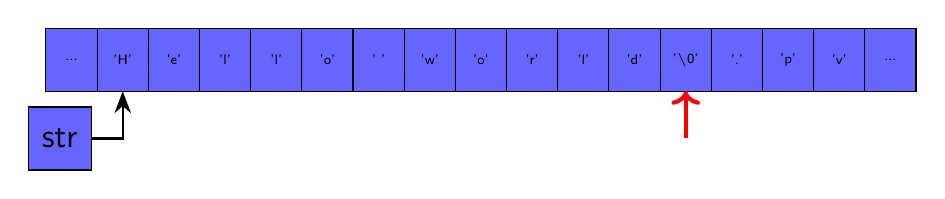
\begin{tikzpicture}[
            node distance=0pt,
            outer sep=0pt,
            cell/.style={
                draw=black, fill=blue!60!white, minimum width=0.65cm, minimum height=0.8cm, text=black, font=\sffamily\tiny, anchor=west
            },
            ptr/.style={
                draw=black, fill=blue!60!white, minimum width=0.8cm, minimum height=0.8cm, text=black, font=\sffamily\large, anchor=center
            }
        ]
            % DÃY Ô NHỚ ĐẦY ĐỦ
            \node[cell] (0) {...};
            \node[cell] (1) at (0.east) {'H'};
            \node[cell] (2) at (1.east) {'e'};
            \node[cell] (3) at (2.east) {'l'};
            \node[cell] (4) at (3.east) {'l'};
            \node[cell] (5) at (4.east) {'o'};
            \node[cell] (6) at (5.east) {' '};
            \node[cell] (7) at (6.east) {'w'};
            \node[cell] (8) at (7.east) {'o'};
            \node[cell] (9) at (8.east) {'r'};
            \node[cell] (10) at (9.east) {'l'};
            \node[cell] (11) at (10.east) {'d'};
            \node[cell] (12) at (11.east) {'\textbackslash 0'};
            \node[cell] (13) at (12.east) {'.'};
            \node[cell] (14) at (13.east) {'p'};
            \node[cell] (15) at (14.east) {'v'};
            \node[cell] (16) at (15.east) {...};

            % --- CON TRỎ STR ---
            % Trỏ vào 'H' (node 1), dịch xuống và sang trái một chút để vẽ mũi tên vuông góc
            \node[ptr] (str) at ([xshift=-0.8cm, yshift=-1.0cm]1.center) {str};

            % MŨI TÊN VUÔNG GÓC TỪ STR LÊN H (node 1)
            \draw[-{Stealth[scale=1.2]}, thick] (str.east) -| (1.south);

            % --- MŨI TÊN ĐỎ CHỈ VÀO \0 (node 12) ---
            % Trỏ thẳng từ dưới lên vào đáy ô \0
            \draw[->, red, line width=1.5pt] (12.south) ++(0, -0.6) -- (12.south);

        \end{tikzpicture}
    \end{center}

    \vspace{-0.2cm}
    \begin{itemize}[label=$\bullet$, itemsep=0.5em]
        \item Để lưu trữ xâu độ dài $N$ ta cần khai báo mảng $N+1$ phần tử.
        \item Hai cách khởi tạo sau là tương đương:
    \end{itemize}

    \vspace{0.1cm} % Thêm chút khoảng cách
    
    % Dùng center để căn giữa toàn bộ khối code này
    \begin{center}
        \begin{tabular}{c c} % Dùng bảng để căn 2 cái code cạnh nhau ngay ngắn giữa màn hình
            \mintinline[fontsize=\scriptsize]{c}{char str[] = "blabla";} & 
            \hspace{0.5cm} % Khoảng cách giữa 2 code
            \mintinline[fontsize=\scriptsize]{c}{char s[]={'b','l','a','b','l','a','\0'};}
        \end{tabular}
    \end{center}
\end{frame}

% --- SLIDE 25: CÁC HÀM NHẬP & XỬ LÝ XÂU ---
% PDF Page 25: Layout 2 cột, cột phải có khung viền
\begin{frame}{Các hàm nhập xâu ký tự và ký tự}
    \small
    \begin{columns}[T]
        % Cột trái: Các hàm nhập
        \begin{column}{0.4\textwidth}
            \begin{itemize}[label=$\bullet$, itemsep=1em]
                \item \texttt{getchar()}
                \begin{itemize}[label=$\circ$, itemsep=0.3em]
                    \item \texttt{c = getchar()}
                \end{itemize}
                \item \texttt{scanf}
                \begin{itemize}[label=$\circ$, itemsep=0.3em]
                    \item \texttt{scanf("\%s", str);}
                \end{itemize}
                \item \texttt{gets()}
                \begin{itemize}[label=$\circ$, itemsep=0.3em]
                    \item \texttt{gets(str);}
                \end{itemize}
            \end{itemize}
        \end{column}

        % Cột phải: Box các hàm xử lý (Viền đen, nền trắng)
        \begin{column}{0.6\textwidth}
            \begin{tcolorbox}[colback=white, colframe=black, boxrule=0.8pt, arc=0pt, left=3pt, right=3pt, top=5pt, bottom=5pt]
                \begin{itemize}[label=$\bullet$, itemsep=0.8em]
                    \item \texttt{strlen(const char s[])}\\
                    \footnotesize{trả về số ký tự của xâu s (không tính ký tự NULL)}
                    
                    \item \texttt{strcmp(const char s1[], const char s2[])}\\
                    \footnotesize{so sánh s1 với s2}
                    
                    \item \texttt{strcpy(char s1[], const char s2[])}\\
                    \footnotesize{sao chép nội dung s2 vào s1}
                    
                    \item \texttt{strcat(char s1[], char s2[])}\\
                    \footnotesize{nối s2 vào s1, sau đó lưu kết quả vào s1}
                \end{itemize}
            \end{tcolorbox}
        \end{column}
    \end{columns}
\end{frame}

% --- SLIDE 26: VÍ DỤ 1 (ĐỀ BÀI) ---
% PDF Page 26: Thay thế ký tự
\begin{frame}{Ví dụ}
    \small
    \begin{itemize}[label=$\bullet$, itemsep=0.8em]
        \item \textbf{Ví dụ 1.} Xây dựng hàm thay thế ký tự trong xâu
        \begin{itemize}[label=$\circ$, itemsep=0.5em]
            \item Hàm có tham số là một xâu ký tự và hai ký tự.
            \item Hàm sẽ duyệt xâu và thay thế tất cả các ký tự thứ nhất trong xâu bằng ký tự thứ hai.
        \end{itemize}
        
        \item Viết chương trình để kiểm tra hàm nói trên:
        \begin{itemize}[label=$\circ$, itemsep=0.5em]
            \item Đọc một xâu không chứa ký tự trắng và hai ký tự, sau đó gọi hàm với các đối số trên và in ra kết quả.
        \end{itemize}
        
        \item \textbf{Ví dụ:}
        \begin{itemize}[label=-]
            \item Đầu vào: "papa", 'p', 'm'
            \item Kết quả: "mama"
        \end{itemize}
    \end{itemize}
\end{frame}

% --- SLIDE 27: VÍ DỤ 1 (CODE FUNCTION) ---
\begin{frame}[fragile]{Ví dụ 1}
    \begin{tcblisting}{
        colback=white, 
        colframe=black, 
        boxrule=0.5pt, 
        arc=2pt,
        listing engine=minted, 
        minted language=c,
        minted options={
            fontsize=\small, % Code ngắn nên để small cho rõ
            breaklines, 
            autogobble, 
            baselinestretch=1,
            tabsize=4
        },
        listing only,
        left=2mm, top=2mm, bottom=2mm
    }
/* function that replace all charaters <replace_what> by <replace_with> in string str */

void replace(char str[], char replace_what, char replace_with)
{
    int i;
    for (i = 0; str[i] != '\0'; ++i)
    {
        if (str[i] == replace_what)
            str[i] = replace_with;
    }
}
    \end{tcblisting}
\end{frame}

% --- SLIDE 28: VÍ DỤ 1 (CODE MAIN) ---
\begin{frame}[fragile]{Ví dụ 1}
    \begin{tcblisting}{
        colback=white, 
        colframe=black, 
        boxrule=0.5pt, 
        arc=2pt,
        listing engine=minted, 
        minted language=c,
        minted options={
            fontsize=\scriptsize, % Code này dùng scriptsize vẫn vừa và dễ đọc hơn tiny
            breaklines, 
            autogobble, 
            baselinestretch=1,
            tabsize=4
        },
        listing only,
        left=2mm, top=2mm, bottom=2mm
    }
#define STRING_LEN 100

int main(void)
{
    char str[STRING_LEN + 1];
    char replace_what, replace_with, tmp;
 
    printf("Please enter a string (no spaces)\n");
    scanf("%100s", str);
 
    printf("Letter to replace: ");
    scanf(" %c", &replace_what);
    // Clear buffer loop
    do { tmp = getchar(); } while (tmp != '\n');
 
    printf("Letter to replace with: ");
    scanf(" %c", &replace_with);
 
    replace(str, replace_what, replace_with);
    printf("The result: %s\n", str);
    return 0;
}
    \end{tcblisting}
\end{frame}

% --- SLIDE 29 (NO BOX VERSION): BÀI TẬP 1 ---
\begin{frame}{Bài tập}
    \small
    \begin{itemize}[label=$\bullet$, itemsep=0.8em]
        \item \textbf{Bài tập 1.} Viết chương trình đọc một xâu ký tự biểu diễn một câu từ người dùng. Sau đó chương trình hiển thị mỗi từ trong câu trên một dòng.
        \begin{itemize}[label=$\circ$, itemsep=0.5em]
            \item Một từ là một dãy các ký tự liên tiếp không chứa ký tự trắng.
        \end{itemize}
        
        \item \textbf{Ví dụ:}
        \begin{itemize}[label=-, itemsep=0.3em]
            \item Đầu vào: \texttt{"The house nextdoor is very old."}
            \item Kết quả:
        \end{itemize}
    \end{itemize}

    \vspace{0.1cm}
    
    % Chỉ là text thuần, thụt dòng vào cho thẳng hàng
    \hspace{1.5cm}
    \begin{minipage}{0.5\textwidth}
        \small
        The\\
        house\\
        nextdoor\\
        ...
    \end{minipage}
\end{frame}

% --- SLIDE 30: BÀI TẬP 2 (DANH SÁCH SV) ---
% PDF Page 30: Bài tập quản lý sinh viên
% --- SLIDE 30 (FIXED - NO BOX): BÀI TẬP 2 ---
% PDF Page 30: Danh sách sinh viên (Style text thuần + gạch chân tên)
\begin{frame}{Bài tập}
    \small
    \begin{itemize}[label=$\bullet$, itemsep=0.8em]
        \item \textbf{Bài tập 2.} Viết chương trình yêu cầu người dùng nhập số lượng sinh viên trong một lớp học, sau đó nhập tên đầy đủ bằng tiếng Việt của mỗi sinh viên. Hiển thị danh sách sinh viên sắp xếp theo tên sinh viên. Ví dụ:
        
        \begin{itemize}[label=$\bullet$, itemsep=0.4em]
            \item Nguyen Bao \underline{Anh}
            \item Tran Quang \underline{Binh}
            \item Vuong Quoc \underline{Binh}
            \item Dao Thi \underline{Ha}
            \item Ngo Anh \underline{Vu}
        \end{itemize}

        \item \textbf{Nâng cao (không bắt buộc):} Hiển thị số lượng lớn nhất các sinh viên cùng tên.
    \end{itemize}
\end{frame}

% --- SLIDE 31: LAB TEST 01 (COUNT WORDS) ---
% PDF Page 31: Đếm số từ trong câu
\begin{frame}[fragile]{Lab test}
    \small
    \textbf{Lab 01. Count words}
    \vspace{0.3cm}
    \begin{itemize}[label=$\bullet$, itemsep=0.8em]
        \item Given a Text, write a program to count the number of words (ignore characters SPACE, TAB, LineBreak) of this Text.
        \item \textbf{Input:} The Text
        \item \textbf{Output:} Write the number of words
    \end{itemize}

    \vspace{0.4cm}
    % Bảng ví dụ đơn giản
    \begin{table}
        \centering
        \small
        \begin{tabular}{|p{0.6\textwidth}|p{0.15\textwidth}|}
            \hline
            \textbf{Input} & \textbf{Output} \\
            \hline
            \texttt{Hanoi University Of Science and Technology} & \texttt{12} \\
            \texttt{School of Information and Communication Technology} & \\
            \hline
        \end{tabular}
    \end{table}
\end{frame}

% --- SLIDE 32: LAB TEST 02 (TEXT REPLACEMENT) ---
% PDF Page 32: Thay thế văn bản
\begin{frame}[fragile]{Lab test}
    \small
    \textbf{Lab 02. Text Replacement}
    \vspace{0.2cm}
    \begin{itemize}[label=$\bullet$, itemsep=0.5em]
        \item Cho văn bản $T$ và 2 mẫu $P1, P2$ đều là các xâu ký tự (không chứa ký tự xuống dòng, độ dài không vượt quá 1000). Hãy thay thế các xâu $P1$ trong $T$ bằng xâu $P2$.
        \item \textbf{Dữ liệu:}
        \begin{itemize}[label=-]
            \item Dòng 1: xâu $P1$
            \item Dòng 2: xâu $P2$
            \item Dòng 3: văn bản $T$
        \end{itemize}
        \item \textbf{Kết quả:} Ghi văn bản $T$ sau khi thay thế
    \end{itemize}

    \vspace{0.2cm}
    \begin{table}
        \centering
        \scriptsize % Dùng scriptsize vì bảng này nhiều chữ
        \begin{tabular}{|p{0.35\textwidth}|p{0.55\textwidth}|}
            \hline
            \textbf{Input} & \textbf{Output} \\
            \hline
            \texttt{AI} \newline \texttt{Artificial Intelligence} \newline \texttt{Recently, AI is a key technology. AI enable efficient operations in many fields.} 
            & 
            \texttt{Recently, Artificial Intelligence is a key technology. Artificial Intelligence enable efficient operations in many fields} \\
            \hline
        \end{tabular}
    \end{table}
\end{frame}

% --- SLIDE 33: CHUYỂN MỤC (SECTION SLIDE) ---
% PDF Page 33: "Con trỏ - pointer"
{
\HUSTUseBackground{theme_hust_oneside.pdf}
\begin{frame}
    \placecontent{0.38\paperwidth}{0.45\paperheight}{0.6\paperwidth}{
        \centering
        \color{HUSTRed}\bfseries\fontsize{24pt}{28pt}\selectfont
        Con trỏ - pointer
    }
\end{frame}
}

\section{Con trỏ}

% --- SLIDE 34: CON TRỎ (FINAL ADJUSTMENT: BLUE & SPACING) ---
\begin{frame}[fragile]{Con trỏ}
    \small
    \begin{itemize}[label=$\bullet$, itemsep=0.5em]
        \item Con trỏ là biến dùng để lưu giá trị một địa chỉ bộ nhớ.
        \item Địa chỉ của biến hoặc mảng.
        \item Được khai báo với ký tự * trước tên.
    \end{itemize}

    \vspace{0.2cm}
    
    % Box cú pháp
    \begin{center}
        \begin{tcolorbox}[colback=white, colframe=black, boxrule=0.5pt, arc=0pt, 
                          left=5pt, right=5pt, top=5pt, bottom=5pt, 
                          standard jigsaw, frame style={dashed}, width=0.6\textwidth, halign=center]
            \ttfamily \large
            Kiểu\_dữ\_liệu \textcolor{blue}{*}tên\_biến;
        \end{tcolorbox}
    \end{center}

    \vspace{0.1cm}

    \begin{itemize}[label=$\bullet$]
        \item Con trỏ \texttt{ptr} được gọi là “trỏ” \textit{point} tới biến c nếu giá trị của nó là địa chỉ của c
    \end{itemize}

    \vspace{0.3cm}
    
    % --- VẼ TIKZ (CĂN CHỈNH CAO ĐỘ, MÀU SẮC, KHOẢNG CÁCH) ---
    \begin{center}
        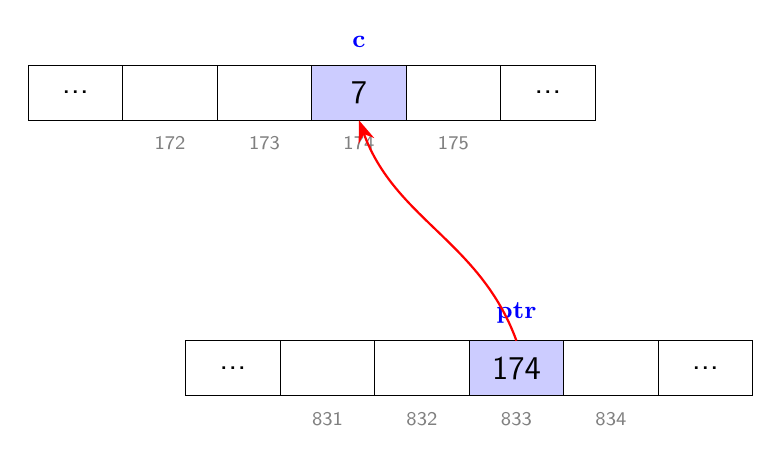
\begin{tikzpicture}[
            node distance=0pt,
            outer sep=0pt,
            % Style ô nhớ: Giảm chiều cao xuống 0.7cm
            cell/.style={
                draw=black,
                minimum width=1.2cm,
                minimum height=0.7cm, % Đã giảm độ cao
                align=center,
                font=\sffamily\large,
                anchor=west,
                fill=white 
            },
            % Style địa chỉ
            addr/.style={
                font=\sffamily\scriptsize,
                text=gray,
                below=0.1cm,
                anchor=north
            },
            % Style tên biến
            varname/.style={
                font=\bfseries\small,
                text=blue,
                above=0.1cm,
                anchor=south
            }
        ]
            % --- DẢI 1: VÙNG NHỚ CHỨA BIẾN C ---
            % Vẫn giữ độ lệch trái 1.5cm
            \node[cell, xshift=-1.5cm, yshift=1.5cm] (c1) {...};
            
            \node[cell] (c2) at (c1.east) {}; 
            \node[addr] at (c2.south) {172}; 

            \node[cell] (c3) at (c2.east) {}; 
            \node[addr] at (c3.south) {173};

            % Ô nhớ 174 chứa biến c
            % Đổi màu fill thành blue!20 (xanh nước biển)
            \node[cell, fill=blue!20] (c_val) at (c3.east) {7}; 
            \node[addr] at (c_val.south) {174};
            \node[varname] at (c_val.north) {c}; 

            \node[cell] (c5) at (c_val.east) {}; 
            \node[addr] at (c5.south) {175};
            
            \node[cell] (c6) at (c5.east) {...};

            % --- DẢI 2: VÙNG NHỚ CHỨA CON TRỎ PTR ---
            % Tăng khoảng cách xuống dưới: below=2.8cm (thay vì 2.0cm)
            % Vẫn giữ độ lệch phải 2.0cm
            \node[cell, below=2.8cm of c1, xshift=2.0cm] (p1) {...};
            
            \node[cell] (p2) at (p1.east) {};
            \node[addr] at (p2.south) {831};

            \node[cell] (p3) at (p2.east) {}; 
            \node[addr] at (p3.south) {832};

            % Ô nhớ 833 chứa ptr
            % Đổi màu fill thành blue!20
            \node[cell, fill=blue!20] (ptr_val) at (p3.east) {174}; 
            \node[addr] at (ptr_val.south) {833};
            \node[varname] at (ptr_val.north) {ptr};

            \node[cell] (p5) at (ptr_val.east) {}; 
            \node[addr] at (p5.south) {834};

            \node[cell] (p6) at (p5.east) {...};

            % --- MŨI TÊN TRỎ ---
            % Vẽ đường cong từ ptr lên c
            \draw[-{Stealth[scale=1.2]}, red, thick] (ptr_val.north) to[out=110, in=-70] (c_val.south);

        \end{tikzpicture}
    \end{center}
\end{frame}

% --- SLIDE 35: TOÁN TỬ THAM CHIẾU & GIẢI THAM CHIẾU ---
\begin{frame}[fragile]{Toán tử tham chiếu (reference) và giải tham chiếu (dereference)}
    \begin{tcblisting}{
        colback=white, 
        colframe=black, 
        boxrule=0.5pt, 
        arc=2pt,
        listing engine=minted, 
        minted language=c,
        minted options={
            fontsize=\small, 
            breaklines, 
            autogobble, 
            baselinestretch=1.1, % Giãn dòng xíu cho dễ đọc
            tabsize=4,
            escapeinside=!! % Dùng cái này nếu muốn chèn LaTeX vào comment
        },
        listing only,
        left=2mm, top=2mm, bottom=2mm
    }
int n;
int* iptr;  /* khai báo iptr là một con trỏ kiểu int */
n = 7;
iptr = &n;

printf(" %d", *iptr); /* Hiển thị '7' */
*iptr = 177;
printf("%d", n);      /* Hiển thị '177' */
iptr = 177;           /* Phép gán không đúng */
    \end{tcblisting}
\end{frame}

% --- SLIDE 36: VÍ DỤ 1 (HÀM TÁCH SỐ) ---
\begin{frame}[fragile]{Ví dụ}
    \small
    \begin{itemize}[label=$\bullet$, itemsep=0.8em]
        \item \textbf{Ví dụ 1.} Viết hàm nhận đối số là một số thực (double) và trả về phần nguyên và phần thập phân của số đó.
        \item Viết chương trình minh họa hàm trên, với số thực được nhập từ người dùng.
    \end{itemize}

    \vspace{0.3cm}
    
    % Box trắng viền xanh dương nhạt (blue!60!white) theo style ảnh gốc
    \begin{tcblisting}{
        colback=white, 
        colframe=blue!60!white, % Đổi màu viền sang xanh
        boxrule=0.8pt, 
        arc=0pt, % Viền vuông góc (arc=0) giống ảnh
        listing engine=minted, 
        minted language=c,
        minted options={
            fontsize=\small, 
            breaklines, 
            autogobble, 
            baselinestretch=1,
            tabsize=4
        },
        listing only,
        left=2mm, top=2mm, bottom=2mm
    }
void split(double num, int* int_part, double* frac_part)
{
    *int_part = (int)num;
    *frac_part = num - *int_part;
}
    \end{tcblisting}
\end{frame}

% --- SLIDE 37: VÍ DỤ 1 (CODE MAIN) ---
\begin{frame}[fragile]{Ví dụ}
    % Box trắng viền xanh dương nhạt (đồng bộ slide 36)
    \begin{tcblisting}{
        colback=white, 
        colframe=blue!60!white, 
        boxrule=0.8pt, 
        arc=0pt, 
        listing engine=minted, 
        minted language=c,
        minted options={
            fontsize=\small, 
            breaklines, 
            autogobble, 
            baselinestretch=1,
            tabsize=4
        },
        listing only,
        left=2mm, top=2mm, bottom=2mm
    }
int main(void) {
    double num, fraction;
    int integer;
    
    printf("Please enter a real number: ");
    scanf("%lf", &num);

    split(num, &integer, &fraction);
    printf("The integer part is %d\n", integer);
    printf("The remaining fraction is %f\n", fraction);

    return 0;
}
    \end{tcblisting}
\end{frame}

% --- SLIDE 38: VÍ DỤ 2 (CODE REPLACE_CHAR) ---
\begin{frame}[fragile]{Ví dụ}
    \small
    \begin{itemize}[label=$\bullet$, itemsep=0.6em]
        \item \textbf{Ví dụ 2.} Viết hàm thay thế ký tự trong xâu với nguyên mẫu hàm:
        \item[] \textcolor{blue}{\textbf{void}} \textbf{replace\_char}(\textcolor{blue}{\textbf{char}} *str, \textcolor{blue}{\textbf{char}} c1, \textcolor{blue}{\textbf{char}} c2);
        \item Hàm sẽ thay thế tất cả các ký tự \textbf{c1} xuất hiện bởi \textbf{c2} trong xâu \textbf{str}.
        \item Minh họa việc sử dụng hàm
    \end{itemize}

    \vspace{0.2cm}
    
    % Box code: Nền xanh rất nhạt (blue!5), viền đen, góc vuông
    \begin{tcblisting}{
        colback=blue!5, 
        colframe=black, 
        boxrule=0.8pt, 
        arc=0pt, 
        listing engine=minted, 
        minted language=c,
        minted options={
            fontsize=\small, 
            breaklines, 
            autogobble, 
            baselinestretch=1,
            tabsize=4
        },
        listing only,
        left=2mm, top=2mm, bottom=2mm
    }
void replace_char(char* str, char c1, char c2)
{
    if (str == NULL)
        return;

    while (*str != '\0') {
        if (*str == c1) {
            *str = c2;
        }
        ++str;
    }
}
    \end{tcblisting}
\end{frame}

% --- SLIDE 39 (FIXED): BÀI TẬP SINH CÂU TỰ ĐỘNG ---
% PDF Page 39: Bài tập mạo từ, danh từ... (image_2441d0.png)
\begin{frame}{Bài tập}
    \small
    \begin{itemize}[label=$\bullet$, itemsep=0.5em]
        \item \textbf{Bài tập 1.} Viết chương trình có khả năng sinh ra các câu tự động sử dụng kỹ thuật lựa chọn dựa trên số ngẫu nhiên.
        \begin{itemize}[label=$\bullet$, itemsep=0.3em]
            \item Chương trình dùng bốn mảng xâu ký tự để lưu trữ \textbf{các mạo từ (article), danh từ (noun), động từ (verb), giới từ (preposition)}.
            \item Câu được tạo ra bằng cách lựa chọn ngẫu nhiên các phần tử trong các mảng trên và ghép lại theo thứ tự: \textbf{mạo từ, danh từ, động từ, mạo từ và danh từ}.
            \item Câu sinh ra cần bắt đầu với ký tự in hoa và kết thúc với dấu chấm.
            \item Chương trình cần sinh ra tối thiểu 10 câu.
        \end{itemize}
        
        \item Ví dụ về các phần tử mảng
        \begin{itemize}[label=$\bullet$, itemsep=0.3em]
            \item mạo từ: "the", "a", "one", "some" and "any";
            \item danh từ: "boy", "girl", "dog", "town" and "car";
            \item động từ: verbs "drove", "jumped", "ran", "walked" and "skipped";
            \item giới từ: "to", "from", "over", "under" and "on".
        \end{itemize}
    \end{itemize}
\end{frame}

% --- SLIDE 40: CHUYỂN MỤC (SECTION SLIDE) ---
% PDF Page 40: "Tham số dòng lệnh"
{
\HUSTUseBackground{theme_hust_oneside.pdf}
\begin{frame}
    \placecontent{0.38\paperwidth}{0.45\paperheight}{0.6\paperwidth}{
        \centering
        \color{HUSTRed}\bfseries\fontsize{24pt}{28pt}\selectfont
        Tham số dòng lệnh
    }
\end{frame}
}

\section{Tham số dòng lệnh}

% --- SLIDE 41: CHƯƠNG TRÌNH VỚI ĐỐI SỐ DÒNG LỆNH ---
% PDF Page 41: Khái niệm
\begin{frame}{Chương trình với đối số dòng lệnh}
    \small
    \begin{itemize}[label=$\bullet$, itemsep=1em]
        \item Các đối số dòng lệnh được định nghĩa trong hàm \texttt{main}.
        \item \texttt{main} bản thân là một hàm như các hàm khác.
        \item Nó có thể nhận các đối số truyền vào (từ dòng lệnh gõ bởi người dùng).
        \item Vai trò của chương trình gọi nó (\textit{the calling function}) trong trường hợp này là hệ điều hành, hoặc một chương trình khác.
    \end{itemize}
\end{frame}

% --- SLIDE 42: NGUYÊN MẪU HÀM MAIN ---
% PDF Page 42: argc và argv
\begin{frame}[fragile]{Nguyên mẫu của hàm main}
    \small
    % Box code cú pháp hàm main
    \begin{center}
        \begin{tcolorbox}[colback=white, colframe=black, boxrule=0.8pt, arc=0pt, 
                          left=5pt, right=5pt, top=5pt, bottom=5pt, width=0.7\textwidth]
            \ttfamily \color{blue} int \color{black} main(\color{blue} int \color{black} argc, \color{blue} char* \color{black} argv[])
        \end{tcolorbox}
    \end{center}

    \vspace{0.3cm}

    \begin{itemize}[label=$\bullet$, itemsep=0.8em]
        \item Khi chúng ta muốn chương trình nhận các đối số tại dòng lệnh, cần định nghĩa hàm \texttt{main} như trên, với:
        
        \begin{itemize}[label=$\bullet$, itemsep=0.5em]
            \item \texttt{argc} chứa số lượng các đối số.
            \item \texttt{argv} là một mảng các con trỏ kiểu \texttt{char} – mảng các xâu ký tự – nhận và lưu trữ các giá trị của các đối số dưới dạng dữ liệu văn bản.
        \end{itemize}
        
        \item Đối số đầu tiên mặc định luôn là tên của chương trình.
    \end{itemize}
\end{frame}

% --- SLIDE 43: ARGC & ARGV (FINAL SIMPLEST ARROW VERSION) ---
\begin{frame}[fragile]{Nguyên mẫu của hàm main}
    \vspace{0.5cm}
    
    \begin{center}
        \large \texttt{int main(int argc, char* argv[])}
    \end{center}

    \vspace{0.5cm}

    \begin{center}
        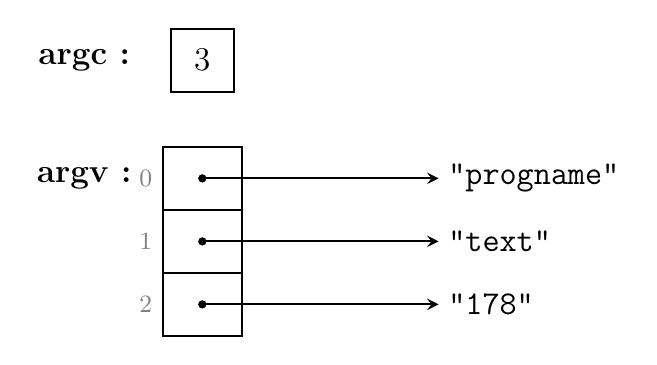
\begin{tikzpicture}[
            % Style cho hộp số (argc)
            numbox/.style={draw, thick, minimum size=0.8cm, font=\large},
            % Style cho ô con trỏ (trống, để vẽ mũi tên từ tâm)
            ptrbox/.style={draw, thick, minimum width=1.0cm, minimum height=0.8cm},
            % Style mũi tên
            arr/.style={->, thick, >=stealth}
        ]
            % --- 1. ARGC ---
            % argc : 3
            \node[font=\large\bfseries] at (0, 0) {argc :};
            \node[numbox] at (1.5, 0) {3};


            % --- 2. ARGV ---
            % argv : (Liệt kê mảng bên dưới)
            \node[font=\large\bfseries] at (0, -1.5) {argv :};
            
            % --- 3. MẢNG CON TRỎ (Xếp dọc) ---
            % Ô thứ 1 (Index 0)
            \node[ptrbox] (p0) at (1.5, -1.5) {};
            \node[left, font=\small, color=gray] at (p0.west) {0}; % Nhãn chỉ số nhỏ bên ngoài

            % Ô thứ 2 (Index 1)
            \node[ptrbox] (p1) at (1.5, -2.3) {};
            \node[left, font=\small, color=gray] at (p1.west) {1};

            % Ô thứ 3 (Index 2)
            \node[ptrbox] (p2) at (1.5, -3.1) {};
            \node[left, font=\small, color=gray] at (p2.west) {2};

            % --- 4. CÁC CHUỖI KÝ TỰ (Bên phải) ---
            \node[right, font=\ttfamily\large] (s0) at (4.5, -1.5) {"progname"};
            \node[right, font=\ttfamily\large] (s1) at (4.5, -2.3) {"text"};
            \node[right, font=\ttfamily\large] (s2) at (4.5, -3.1) {"178"};


            % --- 5. MŨI TÊN TỪ TRUNG TÂM TRỎ RA ---
            % Vẽ dấu chấm tâm cho đẹp (tùy chọn, nhìn giống pointer hơn)
            \fill (p0.center) circle (1.5pt);
            \fill (p1.center) circle (1.5pt);
            \fill (p2.center) circle (1.5pt);

            % Mũi tên đi từ tâm (center) -> chuỗi
            \draw[arr] (p0.center) -- (s0.west);
            \draw[arr] (p1.center) -- (s1.west);
            \draw[arr] (p2.center) -- (s2.west);

        \end{tikzpicture}
    \end{center}
\end{frame}

% --- SLIDE 44: CÁC BƯỚC VIẾT CHƯƠNG TRÌNH ---
% PDF Page 44: Steps
\begin{frame}{Các bước viết chương trình nhận đối số dòng lệnh}
    \small
    \begin{itemize}[label=$\bullet$, itemsep=0.8em]
        \item Viết đúng cú pháp cho hàm \texttt{main}.
        \item Kiểm tra giá trị \texttt{argc} để đảm bảo người dùng nhập đúng số đối số. Nếu sai, hiển thị thông báo cùng hướng dẫn về cú pháp sử dụng chương trình.
        \begin{itemize}[label=$\bullet$, itemsep=0.3em]
            \item VD: \texttt{Hello Hanoi} (1 đối số thực sự), giá trị của \texttt{argc} nên là: $1+1=2$.
        \end{itemize}
        \item Lấy giá trị của các đối số từ mảng \texttt{argv[]}, bắt đầu từ \texttt{argv[1]} và chuyển đổi sang đúng kiểu dữ liệu khi cần thiết.
        \begin{itemize}[label=$\bullet$]
            \item Sử dụng các hàm \texttt{atoi}, \texttt{atol}, \texttt{atof} trong thư viện \texttt{<stdlib.h>}.
        \end{itemize}
        \item Xử lý, tính toán trên các đối số nói trên.
    \end{itemize}
\end{frame}
% --- SLIDE 45: VÍ DỤ 1 (TÍNH DIỆN TÍCH HCN) ---
\begin{frame}[fragile]{Ví dụ}
    \small
    \begin{itemize}[label=$\bullet$, itemsep=0.5em]
        \item \textbf{Ví dụ 1.} Viết chương trình nhận hai số thực làm đối số dòng lệnh, đại diện cho chiều dài và chiều rộng của một hình chữ nhật.
        \item Chương trình dựa trên đó tính toán và in ra diện tích và chu vi của hình chữ nhật.
    \end{itemize}

    \vspace{0.2cm}
    
    % Box code: Nền trắng, viền đen (như slide 28)
    \begin{tcblisting}{
        colback=white, 
        colframe=black, 
        boxrule=0.8pt, 
        arc=0pt, 
        listing engine=minted, 
        minted language=c,
        minted options={
            fontsize=\scriptsize, % Code dài nên dùng scriptsize
            breaklines, 
            autogobble, 
            baselinestretch=1,
            tabsize=4
        },
        listing only,
        left=2mm, top=2mm, bottom=2mm
    }
#include <stdio.h>
#include <stdlib.h>

int main(int argc, char* argv[]) {
    double width, height;
    if (argc != 3) {
        printf("Wrong number of arguments!\n");
        printf("CORRECT SYNTAX: RECT <WIDTH> <HEIGHT>\n");
        return 1;
    }
    
    width = atof(argv[1]);
    height = atof(argv[2]);
    
    printf("The rectangle's area is %f\n", width * height);
    printf("The rectangle's perimeter is %f\n", 2 * (width + height));
    
    return 0;
}
    \end{tcblisting}
\end{frame}

% --- SLIDE 46: BÀI TẬP 1 (ĐẢO NGƯỢC CÂU) ---
% PDF Page 46: Bài tập đảo ngược đối số dòng lệnh
\begin{frame}{Bài tập}
    \small
    \begin{itemize}[label=$\bullet$, itemsep=0.8em]
        \item \textbf{Bài tập 1. Đảo ngược câu}
        \item Viết chương trình cho phép người dùng nhập một câu dưới dạng đối số dòng lệnh (mỗi từ trong câu là một đối số).
        \item Chương trình hiển thị nội dung câu đảo ngược của câu đã nhập.
        
        \item \textbf{Ví dụ: ./inverse I love HUST}
        \item Cho kết quả: \texttt{HUST love I}
    \end{itemize}
\end{frame}

% --- SLIDE 47: BÀI TẬP 2 (GIẢI PHƯƠNG TRÌNH) ---
% PDF Page 47: Giải phương trình bậc 2 từ tham số dòng lệnh
\begin{frame}{Bài tập}
    \small
    \begin{itemize}[label=$\bullet$, itemsep=0.8em]
        \item \textbf{Bài tập 2.} Viết chương trình có tên \textbf{sde} nhận đối số dòng lệnh là các hệ số của một phương trình bậc 2:
        \[ ax^2 + bx + c = 0 \]
        và giải phương trình, in ra màn hình các nghiệm.
        
        \item \textbf{Cú pháp sử dụng:} \texttt{sde a b c}
        
        \item \textbf{Ví dụ:}
        \begin{itemize}[label=$\bullet$, itemsep=0.5em]
            \item \texttt{./sde 1 2 1}
            \item Cho kết quả: \texttt{x1 = x2 = -1}
        \end{itemize}
    \end{itemize}
\end{frame}

\end{document}